\section{Planning}
\frame{\tableofcontents[currentsection, hideothersubsections]}

\begin{frame}
\frametitle{How to control a robot from START to +1 (GOAL)?}
\begin{figure}
    \centering
    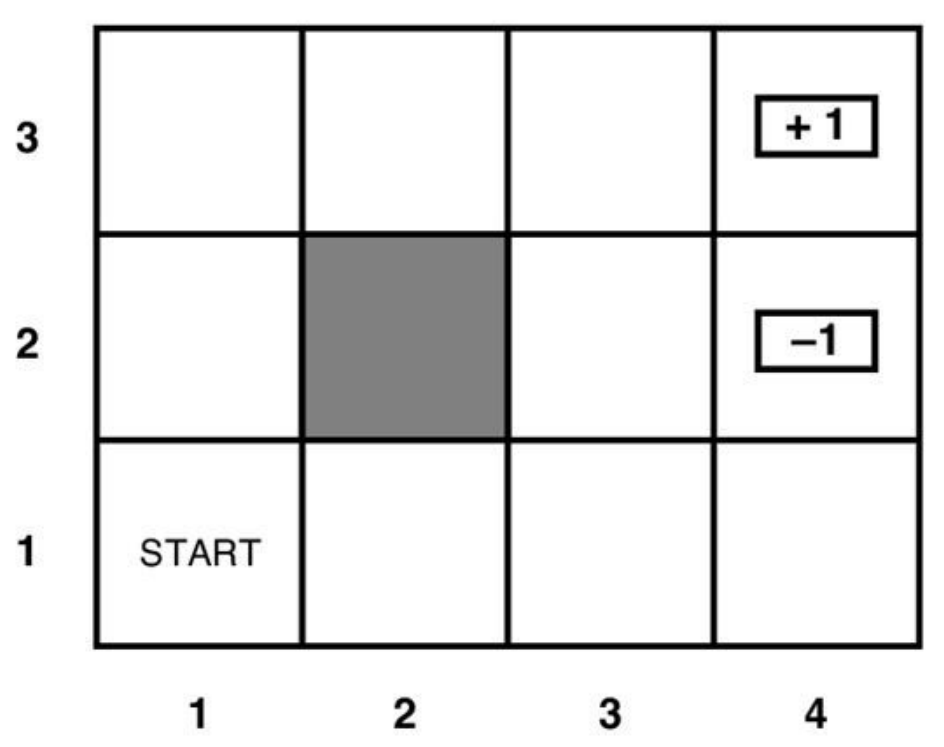
\includegraphics[scale=0.25]{grid_world_only}
\end{figure}
\pause

\begin{itemize}
  \item Wall following? right or left? who decides? \pause
  \item What if START can be in any grid? \pause
  \item What if actions are uncertain?
\end{itemize}
\end{frame}

\begin{frame}
\frametitle{How to control a robot from START to +1 (GOAL)?}
\begin{figure}
    \centering
    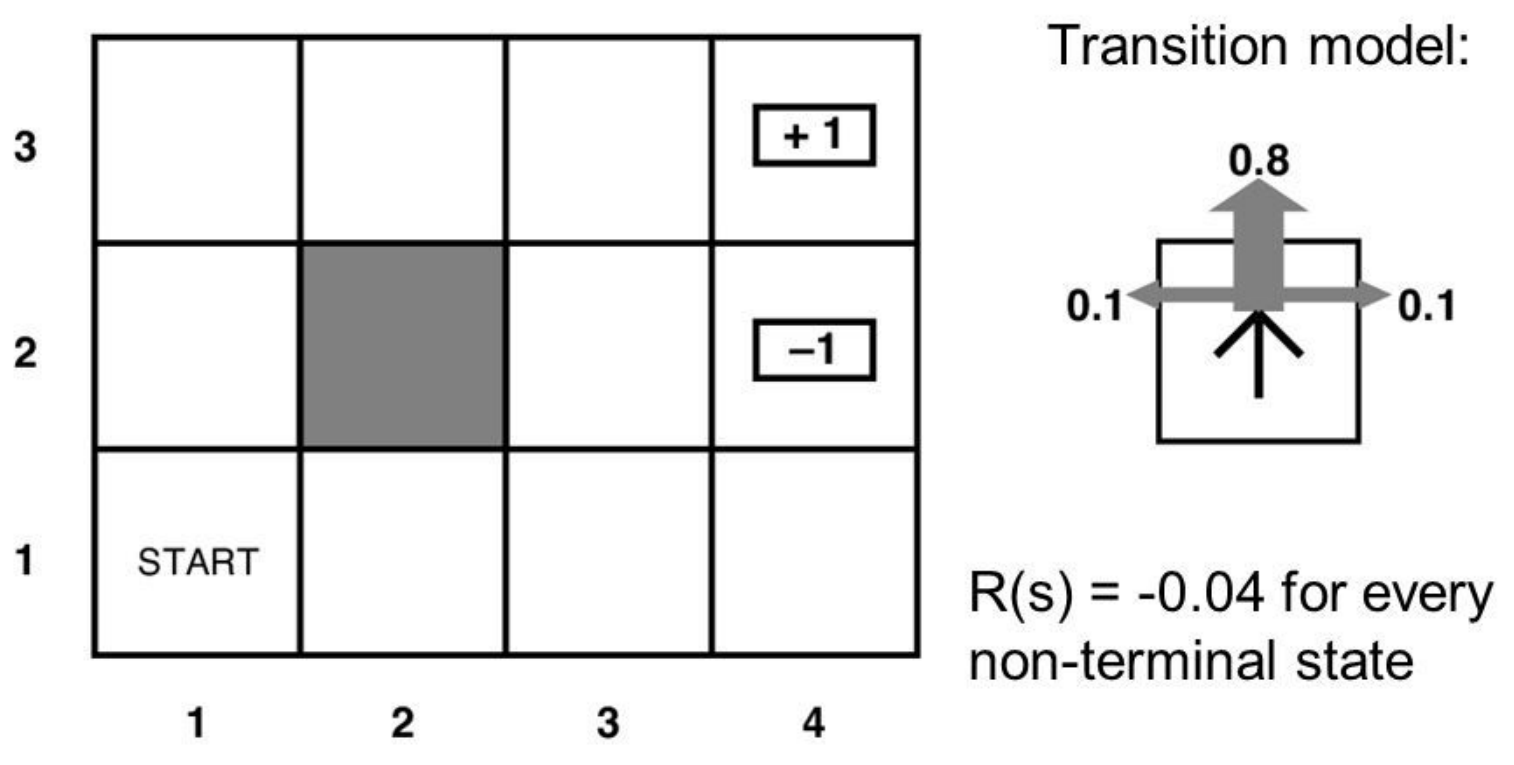
\includegraphics[scale=0.25]{grid_world_with_transition}
\end{figure}
\pause

\begin{itemize}
  \item Given environment model, one possible solution: \\
  \textbf{MDP planning}: sequential decision making under action uncertainty
\end{itemize}
\end{frame}

\begin{frame}
\frametitle{MDP: Markov Decision Process}
\begin{figure}
    \centering
    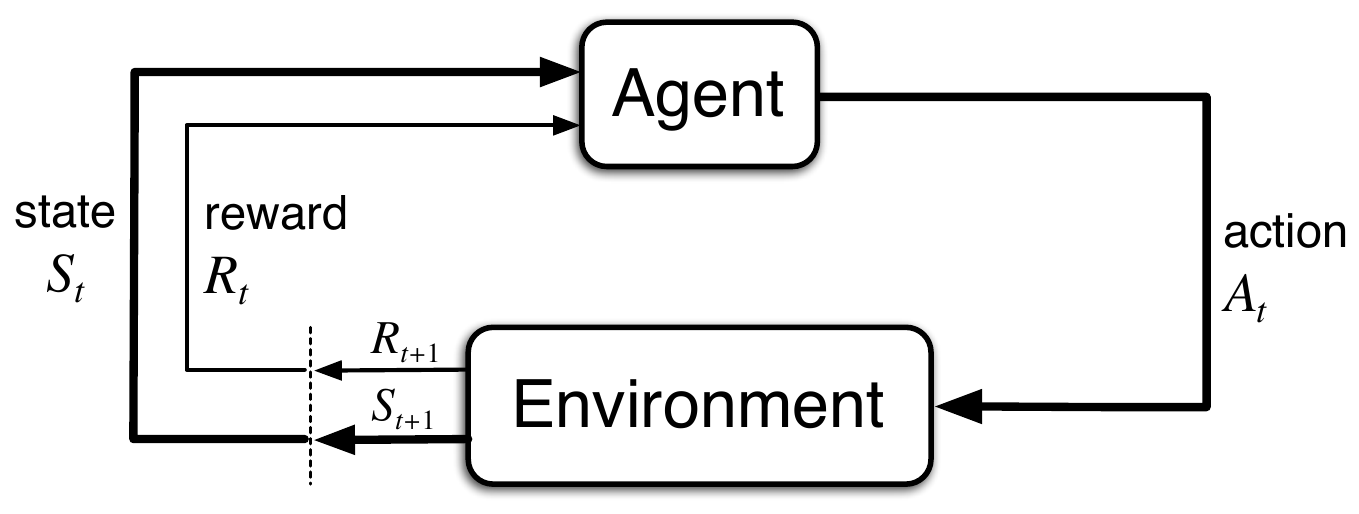
\includegraphics[scale=0.25]{agent_environment_rl_intro_p60}
\end{figure}
\pause
\begin{columns}
  \column{0.5\textwidth}
    $MDP = (S, A, T, R, \gamma)$ ... the model \pause
    \begin{itemize}
      \item $S$ is a set of states
      \item $A$ is a set of actions \pause
      \item $T(s,a,s') = P(s'| s, a)$ \\ is a transition function \pause
      \item $r:(s,a,s') \mapsto \mathbb{R}$ \\ is a reward function \pause
      \item $\gamma \in [0,1]$ is a discount factor
    \end{itemize}
    \pause
  \column{0.5\textwidth}
    \textbf{Agent's goal in MDP planning:}\\
    to maximize the return, $\mathcal{R}$,\\
    (i.e. the expected cumulative reward) \\
    \begin{align*}
      \mathcal{R}_t & = r_{t+1} + \gamma~r_{t+2} + \gamma^2~r_{t+3} + \ldots  \\
      & = \sum_{k=0}^{\infty} \gamma^k~r_{t+k+1}
    \end{align*}
\end{columns}
\end{frame}

\begin{frame}
\frametitle{MDP Planning: Value Function and Policy (Plan)}
\textbf{(State) value function:} the goodness of a state
\begin{align*}
V(s) & = \mathbb{E}[\mathcal{R}_t | S_t = s] \\
& = \mathbb{E} [r_{t+1} + \gamma~r_{t+2} + \gamma^2~r_{t+3} + \ldots | S_t = s] \\
& = \mathbb{E} [r_{t+1} + \gamma~ (r_{t+2} + \gamma~r_{t+3} + \ldots | S_t = s)] \\
& = \mathbb{E} [r_{t+1} + \gamma~ (\mathcal{R}_{t+1} | S_t = s)] \\
& = \mathbb{E} [r_{t+1} + \gamma~V(S_{t+1}| s)]
\end{align*}
\pause

\textbf{A policy (plan)} maps every state to an action, $\pi: s \mapsto a$, \\
generally, $\pi (a|s) = P[A_t = a|S_t = s]$
\end{frame}

\begin{frame}
\frametitle{MDP Planning: From Value Function To Policy}
$\pi = greedy(V)$ \\
Recall: the agents' goal is to maximize the expected cumulative return

\begin{columns}
  \column{0.5\textwidth}
    \begin{figure}
        \centering
        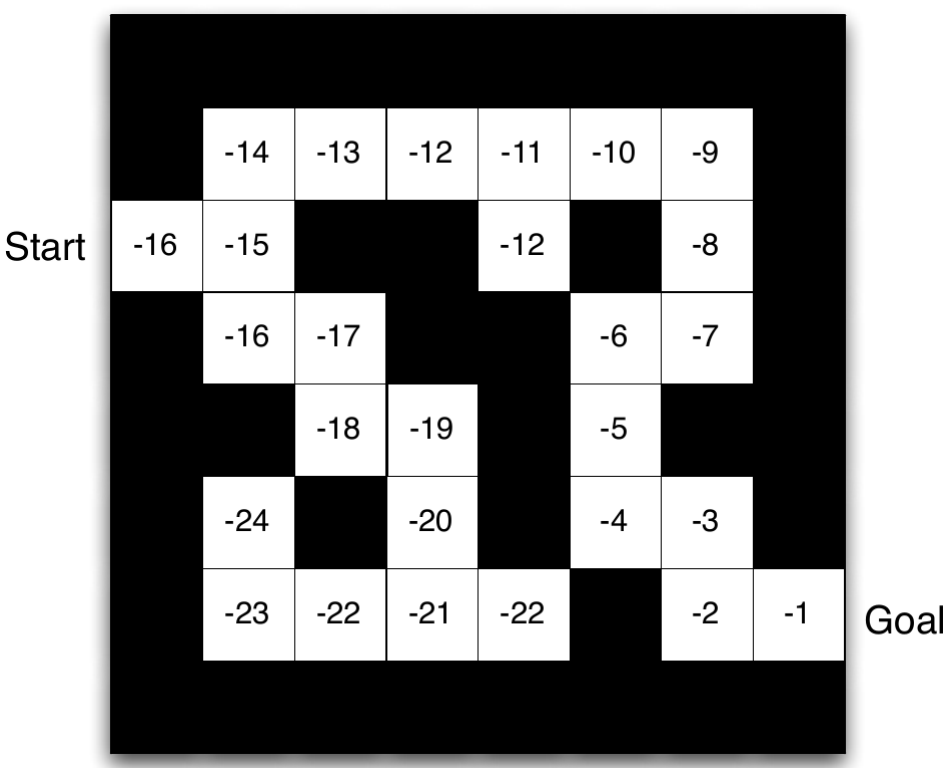
\includegraphics[scale=0.25]{value_function_example_silver_course}
        \caption{a (state) value function}
    \end{figure}

  \column{0.5\textwidth}
    \begin{figure}
        \centering
        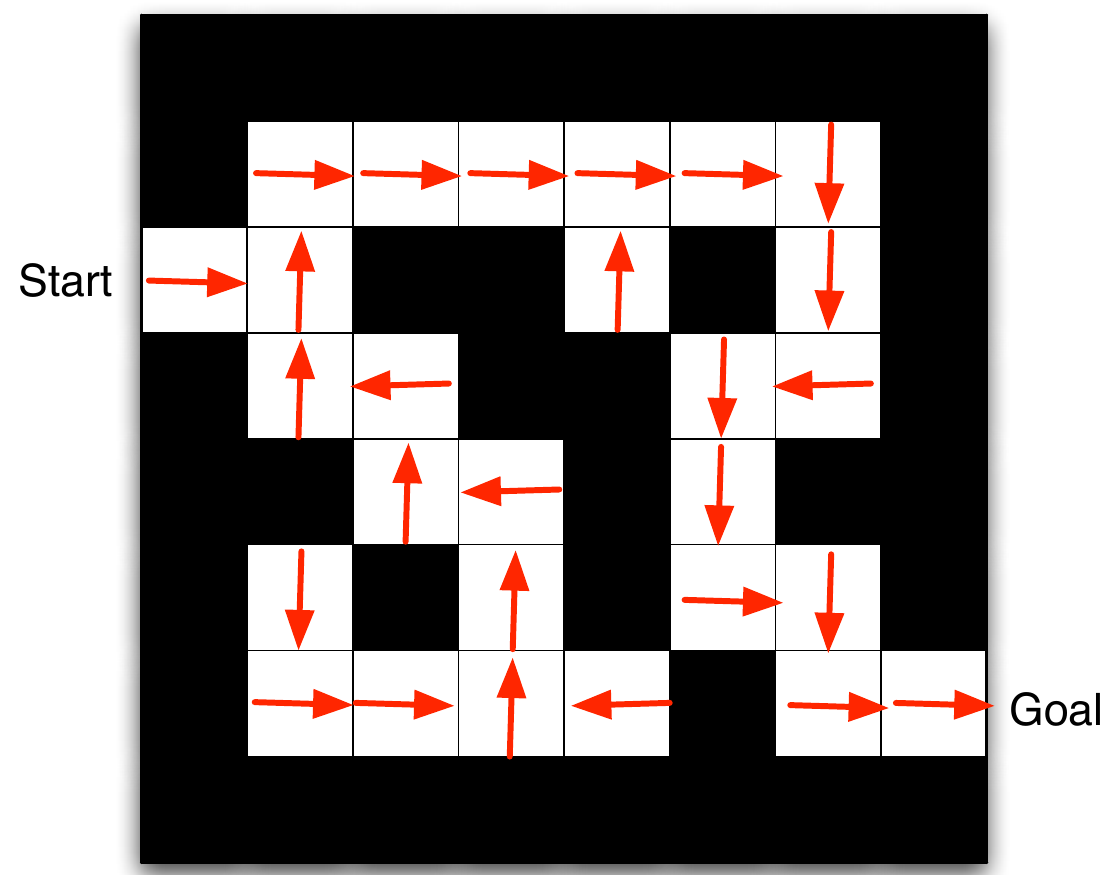
\includegraphics[scale=0.20]{policy_example_silver_course}
        \caption{a policy (plan)}
    \end{figure}
\end{columns}
\end{frame}

\begin{frame}
\frametitle{MDP Planning: Value Iteration (Dynamic Programming)}
\begin{figure}
    \centering
    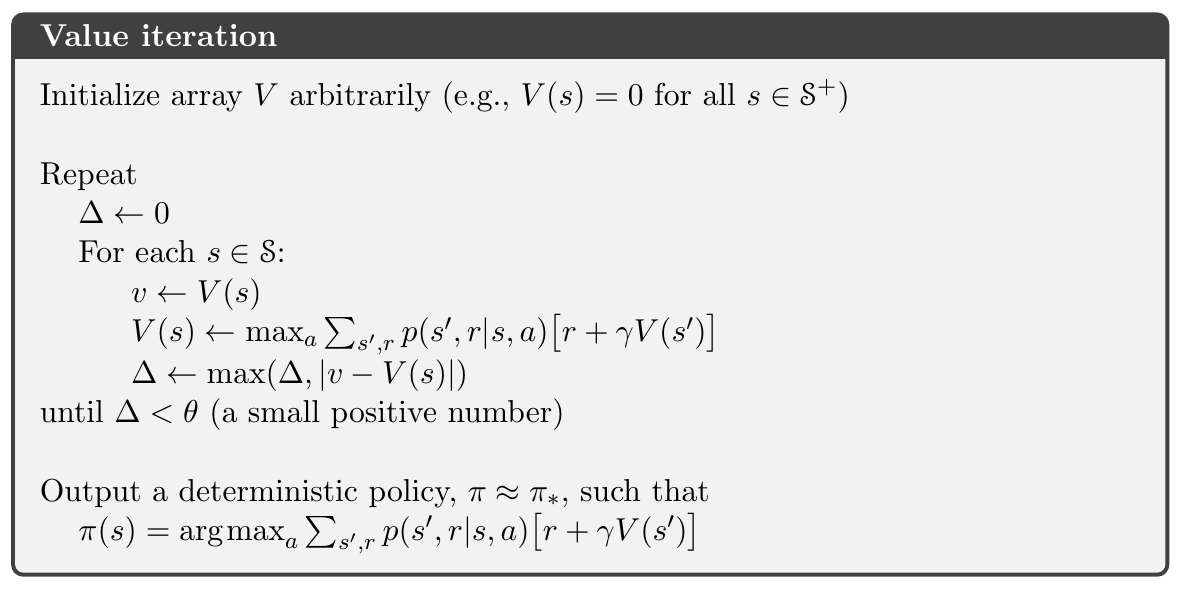
\includegraphics[scale=0.4]{value_iter_rl_intro_p92}
\end{figure}
\end{frame}

\begin{frame}
\frametitle{MDP Planning: Value Iteration Example}
\begin{figure}
    \centering
    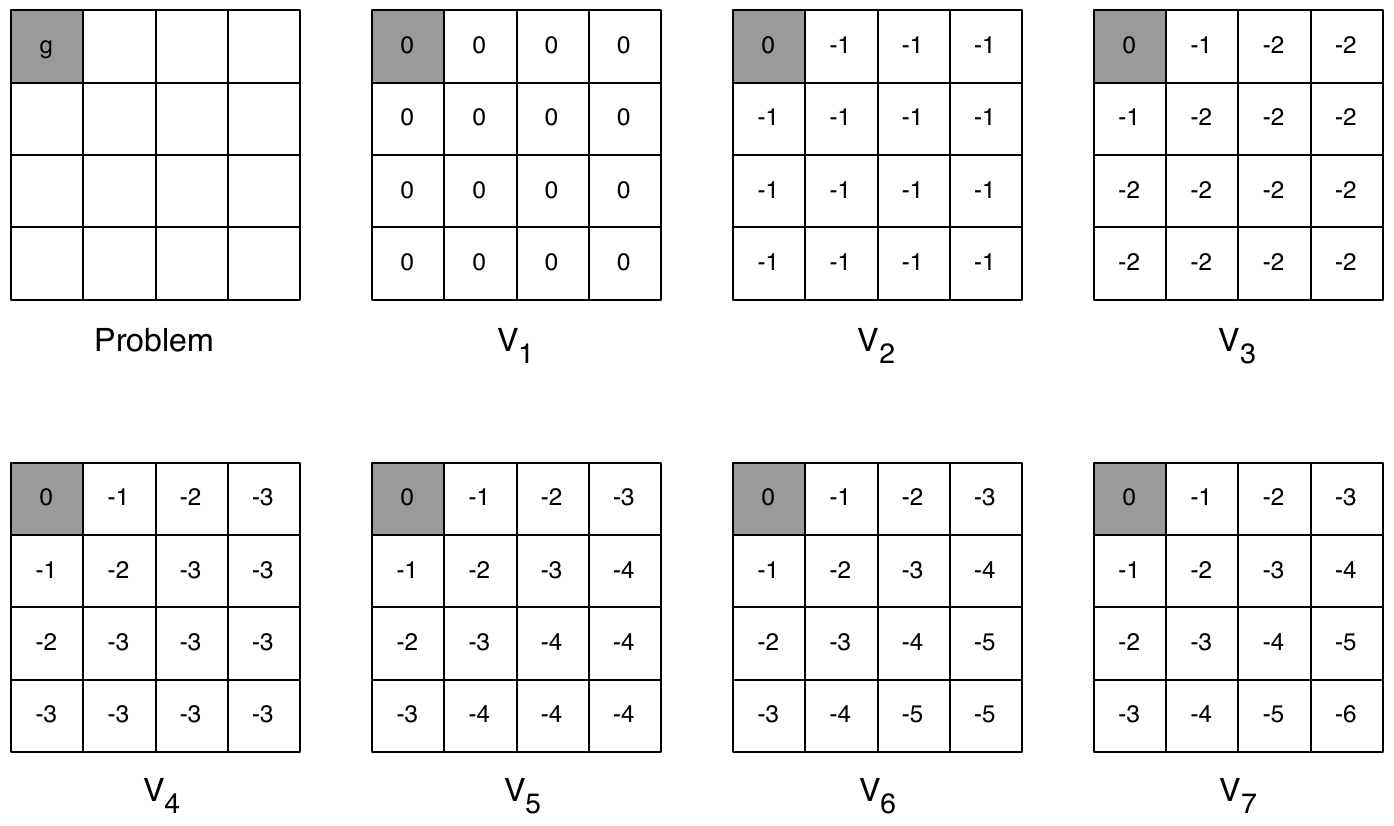
\includegraphics[scale=0.3]{value_iter_shortest_path_silver_course_2}
\end{figure}
\end{frame}

\begin{frame}
\frametitle{MDP Planning}
Iterations toward an optimal policy (plan)
\begin{figure}
    \centering
    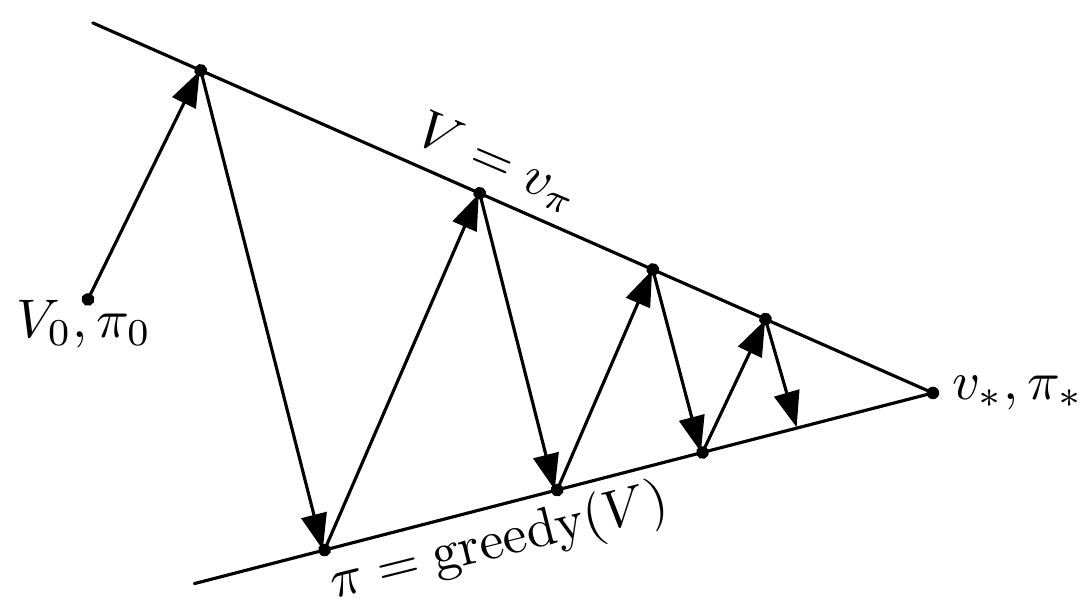
\includegraphics[scale=0.35]{gpi_rl_intro_p96}
\end{figure}
\end{frame}

\begin{frame}
\frametitle{MDP Planning}
\begin{figure}
    \centering
    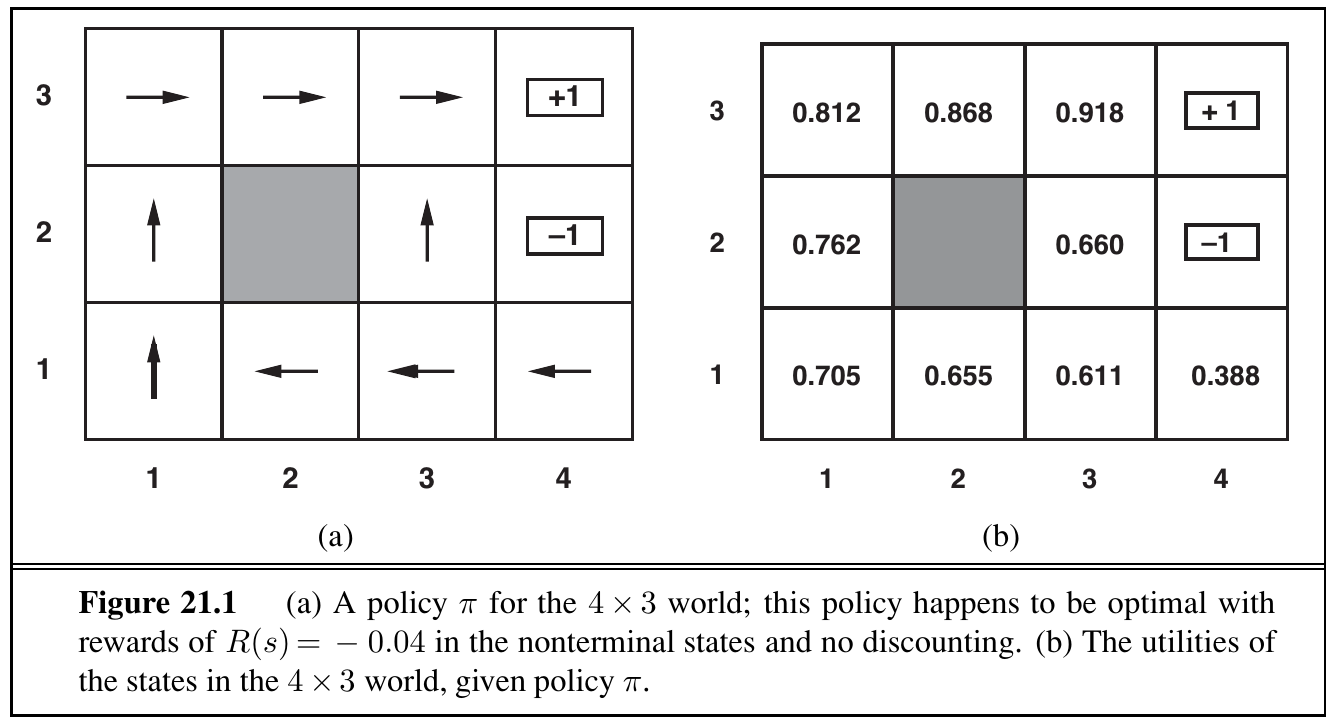
\includegraphics[scale=0.35]{policy_grid_world_aima_p832}
\end{figure}
\end{frame}